\documentclass[hyperref={bookmarks=false},aspectratio=169]{beamer}
\usepackage[utf8]{inputenc}

% ---------------  Define theme and color scheme  -----------------
\usetheme[minimal]{Caltech}  % 3 options: minimal, sidebarleft, sidebarright

%\setbeamertemplate{footline}[frame number]

% ------------  Information on the title page  --------------------
\title[A Swampland Constraint on Gravitational Collapse]
{\bfseries{A Swampland Constraint on Gravitational Collapse}}

\subtitle{Master's thesis by Himanshu Chaudhary}

\author[Himanshu Chaudhary]
{\textbf{Advisor}: Chethan Krishnan\inst{1}
\and \\
\textbf{Committe members}:
Prasad Hegde\inst{1} \and Sachindeo Vaidya\inst{1}
} 
% {Mischief\inst{1} \and Managed\inst{2}}

\institute[IISc]
{
  \inst{1}
  Center for High Energy Physics\\
  Indian Institute of Science
  % \and
  % \inst{2}
  % Department of Student Pranks\\
  % California Institute of Technology
}

\date[IISc, 2020]
{1st July, 2020}
% {International Conference on University Pranks\\April 1st, 2014}
%------------------------------------------------------------

%------------------------------------------------------------
%The next block of commands puts the table of contents at the 
%beginning of each section and highlights the current section:

% \AtBeginSection[]
% {
%   \begin{frame}
%     \frametitle{Table of Contents}
%     \tableofcontents[currentsection]
%   \end{frame}
% }
%------------------------------------------------------------


\begin{document}

\frame{\titlepage}  % Creates title page

% %---------   table of contents after title page  ------------
% \begin{frame}
%   \frametitle{Table of Contents}
%   % \tableofcontents
% \end{frame}
% %---------------------------------------------------------


\section{Caltech student traditions}

%---------------------------------------------------------
%Changing visivility of the text
\begin{frame}
  \frametitle{Millikan pumpkin-drop experiment}
  Every Halloween, Dabney House conducts the infamous ``Millikan pumpkin-drop experiment'' from the top of Millikan Library, the highest point on campus.

  \begin{itemize}
    \item<1-> A claim was once made that the shattering of a pumpkin frozen in liquid nitrogen and dropped from a sufficient height would produce a triboluminescent spark.
    \item<2-> This yearly event involves a crowd of observers, who try to spot the elusive spark.
    \item<3-> The title of the event is an oblique reference to the famous Millikan oil-drop experiment which measured $e$, the elemental unit of electrical charge.
  \end{itemize}

\end{frame}

%---------------------------------------------------------


%---------------------------------------------------------
%\begin{frame}  % Example of the \pause command
%This slide is to test mathematical formulas \pause
%
%$$E=mc^2$$ \pause
%
%as well as the ``pause'' functionality
%\end{frame}
%---------------------------------------------------------

\section{Caltech student pranks}

%---------------------------------------------------------
%Highlighting text
\begin{frame}
  \frametitle{Caltech student pranks}

  This is a brief introduction of \alert{Caltech pranks}.

  \begin{block}{Definition}
    Prank: a practical joke or mischievous act
  \end{block}

  \begin{alertblock}{Axiom}
    Caltech pranks are a key part of the institute's history and identity.
  \end{alertblock}

  \begin{examples}
    See the next slide for a prank example.
  \end{examples}
\end{frame}
%---------------------------------------------------------


%---------------------------------------------------------
%Two columns
\begin{frame}
  \frametitle{Hollywood sign}

  \begin{columns}

    \column{0.45\textwidth}

    \begin{figure}
      \centering
      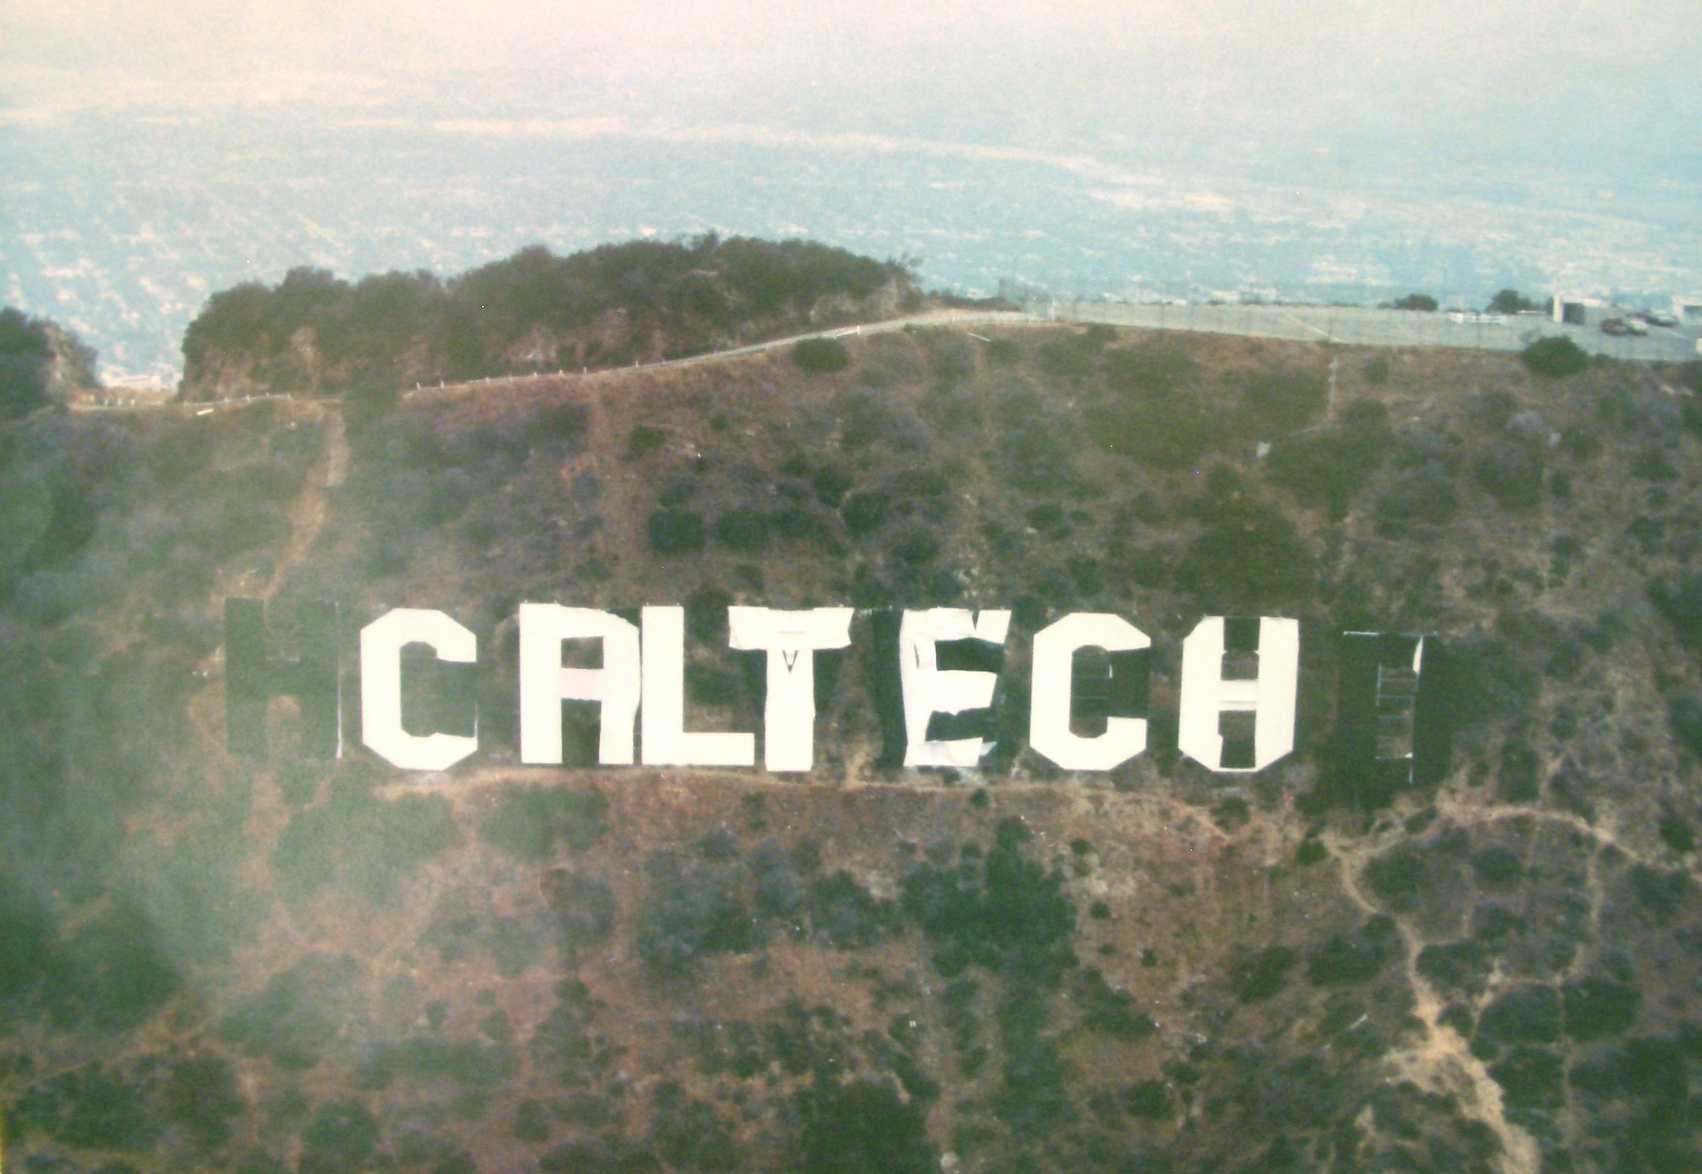
\includegraphics[width=\columnwidth]{./figures/hollywood_caltech.jpg}
      \caption{``Hollywood is still mad about that,'' says Autumn Looijen, author of \emph{Legends of Caltech III: Techer In the Dark.} \tiny{(Photo downloaded from: http://brennen.caltech.edu/autobiography/automaster2.htm)}}
      \label{fig:hollywood_prank}
    \end{figure}


    \column{0.55\textwidth}
    In May 1987, undergraduates from Page and Ricketts houses combined forces (and several hundred dollars) to purchase enough black and white plastic, transformed the Hollywood sign to read ``Caltech''.

    \small{(Reference: http://www.admissions.caltech.edu/pranks)}

  \end{columns}
\end{frame}
%---------------------------------------------------------


\end{document}